% Chapter 1

l\chapter{Introduction} % Main chapter title

\label{Introduction} % For referencing the chapter elsewhere, use \ref{Chapter1} 

%----------------------------------------------------------------------------------------

% Define some commands to keep the formatting separated from the content 
\newcommand{\keyword}[1]{\textbf{#1}}
\newcommand{\tabhead}[1]{\textbf{#1}}
\newcommand{\code}[1]{\texttt{#1}}
\newcommand{\file}[1]{\texttt{\bfseries#1}}
\newcommand{\option}[1]{\texttt{\itshape#1}}

%----------------------------------------------------------------------------------------

\section{Modern Cosmology}
 
\subsection{The Big Bang Theory}
The basis for modern cosmology relies on several fundamental assumptions stemming from observation, the chief of which is the Big Bang Model. Following Hubble's discovery of a relation between distances to galaxies and their recessional velocities, the \emph{Copernican Principle} leads to the conclusion that in the past, objects in the universe were much closer together. His observations gave rise to the Lemaitre's Hubble Law, 
\begin{equation}
v  \varpropto d 
\label{eq:HubbleLaw}
\end{equation}
This suggests that at some point in the past, the universe was much smaller than it is at present, the conservation of energy then implies that at some point in the past, the universe must have been an incredibly hot, dense environment. Using general relativity, the extrapolation backwards in time yields a singularity of infinite density and temperature, which is commonly called the \emph{Big Bang}
\par Another assumption stemming from observation is that of isotropy. Based on observation, there appears to be no favoured direction in the universe, since distributions of distant galaxies and other extragalactic sources seem to be evenly distributed across the sky. Perhaps the most spectacular example of this isotropy is the presence of the \emph{Cosmic Microwave Background}. 
\par Discovered in 1964 \citep{Penzias:65}, it was noticed that there was isotropic black-body radiation at $T \approx \SI{2.7}{\kelvin}$. Since the peak of this radiation is in the microwave section of the electromagnetic spectrum, it was termed the \emph{Cosmic Microwave Background}. 
\begin{figure}[h]
\centering
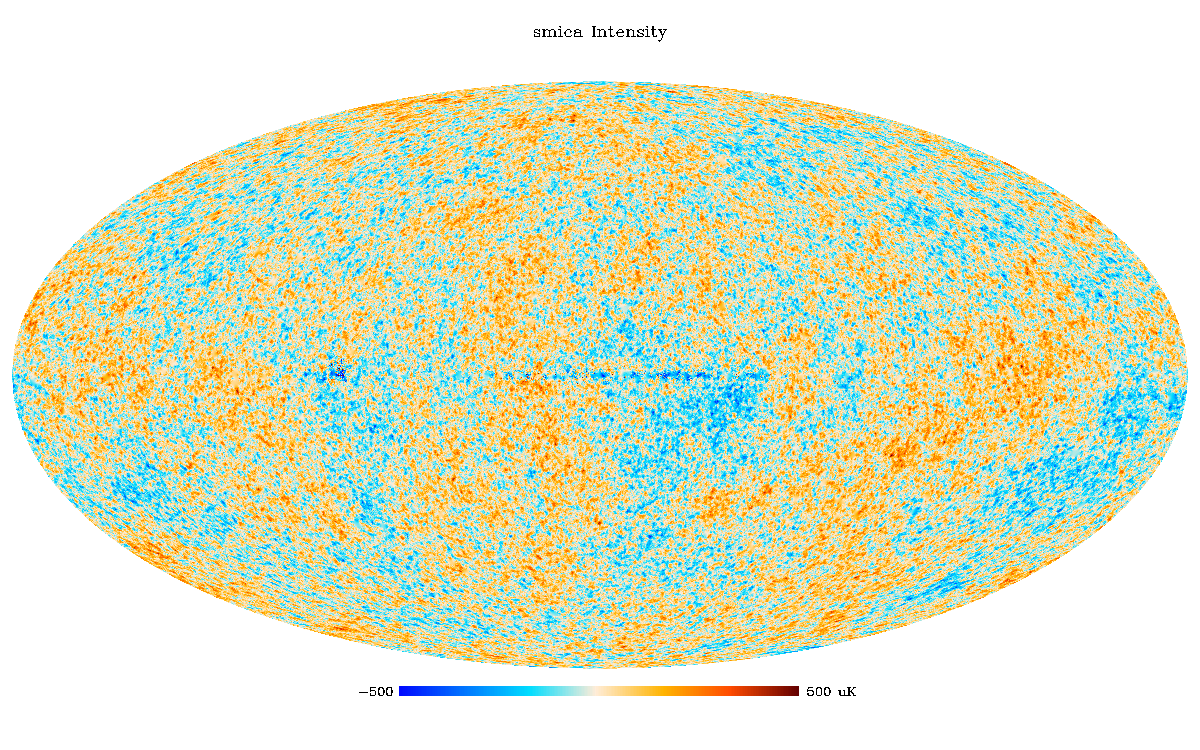
\includegraphics[scale=0.25]{../Images/CMB_smica_tsig.png} 
\label{CMB Map}
\caption{\emph{Planck} Satellite Full Sky CMB Map}
\end{figure}
This picture, whilst useful at a basic level, presents problems when examined more closely. As it stands, the edges of the observable universe at present are too far away from each other to be causally connected. What accounts for the observed homogeneity and isotropy then, if entire areas of the universe cannot affect each other, or communicate information, and so cannot mix? Measurements of the CMB also indicate that the universe is spatially flat, but the initial conditions required to maintain this state are incredibly specific. There is no reason to suggest that these conditions should be preferentially selected over any others. If the conditions for homogeneity and isotropy are maintained sufficiently to allow this, how then does the observed large scale structure of the universe come about? There are also addition problems arising from particle physics, including considerations regarding magnetic monopoles and gravitinos, which have to be satisfied.

\subsection{Inflation}
The most commonly held solution to these problems is the theory of \emph{cosmological inflation}\cite{Linde:07}. This is a period at a very early epoch of the universe where the expansion rate of the universe is exponentially large. This expansion allows for quantum density fluctuations to grow into real density fluctuations, whilst still maintain their causal connection at very early times. 